\documentclass[tikz,border=8pt]{standalone}
\usetikzlibrary{arrows.meta,positioning,fit}
\begin{document}
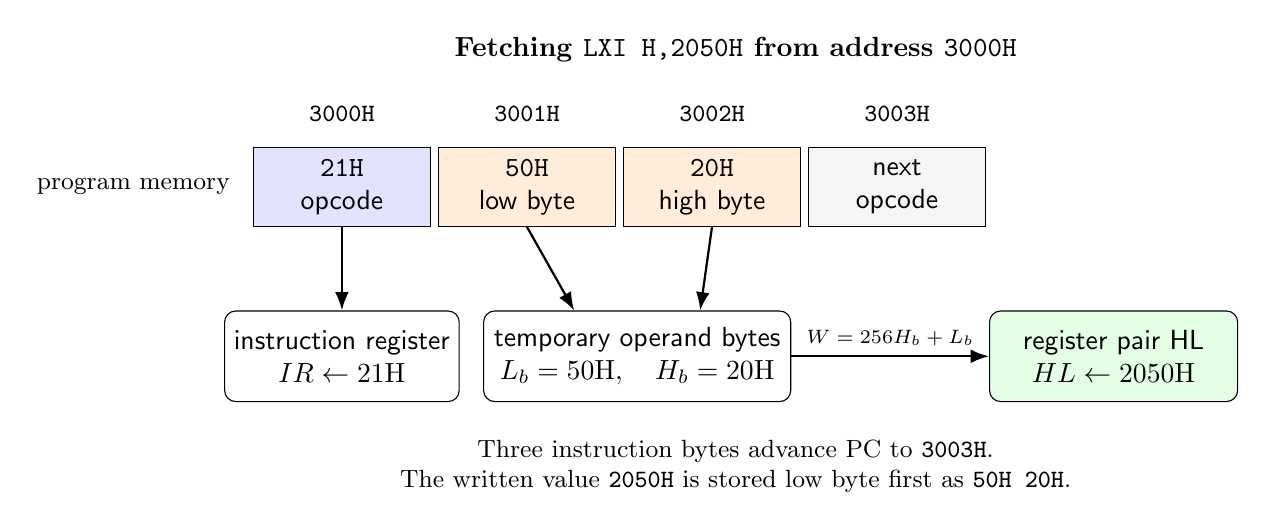
\begin{tikzpicture}[
  font=\sffamily,
  >=Latex,
  cell/.style={draw,minimum width=2.25cm,minimum height=1.0cm,align=center},
  flow/.style={->,thick},
  box/.style={draw,rounded corners,minimum height=1.15cm,align=center}
]
\node[font=\bfseries] at (5.0,4.05) {Fetching \texttt{LXI H,2050H} from address \texttt{3000H}};

\node[font=\small,anchor=east] at (-1.30,2.30) {program memory};
\node[cell,fill=blue!11] (c0) at (0,2.30) {\texttt{21H}\\opcode};
\node[cell,fill=orange!15] (c1) at (2.35,2.30) {\texttt{50H}\\low byte};
\node[cell,fill=orange!15] (c2) at (4.70,2.30) {\texttt{20H}\\high byte};
\node[cell,fill=gray!8] (c3) at (7.05,2.30) {next\\opcode};
\node[above=2mm of c0,font=\ttfamily\small] {3000H};
\node[above=2mm of c1,font=\ttfamily\small] {3001H};
\node[above=2mm of c2,font=\ttfamily\small] {3002H};
\node[above=2mm of c3,font=\ttfamily\small] {3003H};

\node[box,minimum width=2.9cm] (ir) at (0,0.15) {instruction register\\$IR\leftarrow21\mathrm{H}$};
\node[box,minimum width=3.9cm] (tmp) at (3.75,0.15) {temporary operand bytes\\$L_b=50\mathrm{H},\quad H_b=20\mathrm{H}$};
\node[box,minimum width=3.15cm,fill=green!10] (hl) at (9.8,0.15) {register pair HL\\$HL\leftarrow2050\mathrm{H}$};

\draw[flow] (c0.south) -- (ir.north);
\draw[flow] (c1.south) -- ([xshift=-8mm]tmp.north);
\draw[flow] (c2.south) -- ([xshift=8mm]tmp.north);
\draw[flow] (tmp) -- node[above,font=\scriptsize] {$W=256H_b+L_b$} (hl);

\node[font=\small,align=center] at (5.0,-1.25)
 {Three instruction bytes advance PC to \texttt{3003H}.\\The written value \texttt{2050H} is stored low byte first as \texttt{50H 20H}.};
\end{tikzpicture}
\end{document}
